
\chapter{Распутинщина}


Говоря о России в преддверии Первой мировой войны многие затрудняются с полноценной характеристикой ситуации в стране. В таких случаях на помощь обычно приходит ёмкое словцо, которое, как кажется на первый взгляд, способно описать весь раздрай внутри и вокруг царского двора, всю непоследовательность решений и абсурдных назначений.

Распутинщина.

На деле же - это, хоть и весьма специфичный, но раздутый эпизод той эпохи. И реальное его значение часто преувеличивается.

Появившийся при царском дворе ещё в 1905 году, старец Григорий приобрёл удивительную популярность после 1911 года. "Странным" образом это совпало с падением влияния Совета Министров и распылением власти его председателя.

Следующему по очереди премьеру В.Н. Коковцеву, назначенному после смерти П.А. Столыпина, жена Николая II Александра Фёдоровна скажет "не заслоняйте императора". Так новых премьеров предупреждали от ошибок активного Петра Аркадьевича. После инцидента с западными земствами император изменил свое отношение к Столыпину и посчитал его действия угрозой его самодержавной власти.

Начиная с председательства Коковцова, император всё чаще стал вмешиваться в министерские назначения, на Совет министров взваливали всё новые и новые мелкие поручения, а личное обсуждение важных вопросов императором и премьером прекратилось вовсе.

В подобных обстоятельствах в поле зрения общества и появляется Григорий Распутин. Он был не единственным среди неофициальных приближённых императора, однако внимания привлекал гораздо больше, чем Митька Козельский или французский маг Филипп Низье. Да и отдельные аристократические обществ, вроде кружков Штюрмера и Римского-Корсакова, также влиявшие на царя, никого не удивляли. Другое дело - сибирский мужик, устраивающий оргии на своей квартире, одевающийся и ведущий себя в высшей степени вызывающе. 

\begin{figure}[h!tb] 
	\centering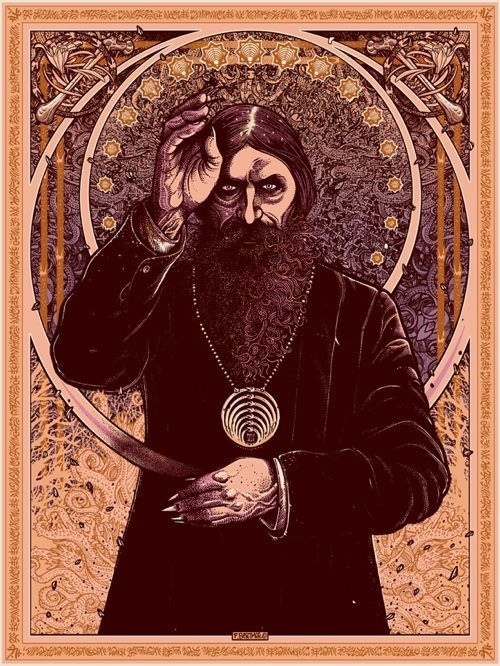
\includegraphics[scale=0.3]{Data/Rasputinschina/sUranFzq1iQ.jpg}
	%	\label{fig:scipion} % Unique label used for referencing the figure in-text\end{document}
	%	%\addcontentsline{toc}{figure}{Figure \ref{fig:placeholder}} % Uncomment to add the figure to the table of contents%----------------------------------------------------------------------------------------
	\caption{Вольная трактовка внешности Распутина.}%	CHAPTER 2
\end{figure}

Есть версия, что влияние Распутина и вовсе было иллюзорным, но это заблуждение. Преувеличенным - в общественном сознании - да. Однако, не совсем также ясно, насколько серьезно он мог повлиять на царя, так как не каждое его требование или совет беспрекословно исполнялись. Да и о влиянии Распутина мы знаем, по большей части, со слов самого Распутина, постоянно себя расхваливающего.

Широкая народная молва вокруг него росла не только благодаря самому старцу Григорию. Ситуация усугублялась состоянием политического системы страны, сложившейся после 1911 года.

В условиях, когда Совет министров утрачивает своё значение и сокращается сфера публичности принятия решений, возможности прямого воздействия на императора сокращаются. В подобных условиях создаются различные теневые каналы, позволяющие влиять на императора без общественной огласки. Те же кружки кружки Штюрмера и А.А. Римского-Корсакова, также как и Распутин, влияли на царя, но не имели политической программы, а решали свои частные задачи и пополняли собственный карман.

О том, насколько влиятелен был Распутин, может сказать его тактика решения многочисленных прошений, которые подавали ему жалобщики в квартире на Гороховой улице. Он никогда не отказывался помочь и по мере своих сил пытался выполнить просьбу каждого, кто к нему приходил, отрабатывая плату. Большая часть решений требовала государственного вмешательства, поэтому, после обработки просьб, Распутин относил записочки просителей нужным человечкам. Дальше все зависело от степени пугливости кадра. Так, например, когда старец пришёл к А.Н. Наумову (министр земледелия) и попытался загипнотизировать, тот, не долго думая, спустил старца с лестницы.

Распутин не является интересным сам по себе, хотя личность он действительно необычная. Он является симптомом, маркером ухода власти в теневое поле, недоступное общественности. Отсюда и появляются повышенное внимание к мистическим старцам, шпиономания и сомнения в верховной власти, которая попросту не говорит о том, какие решения принимает. Ведь неведение обостряет обстановку в обществе куда сильнее, чем самые спорные, но хотя бы проводимые публично, преобразования.

Автор Илья Агафонов. Оригинал \url{https://vk.com/wall-162479647_142075}

\#Агафонов@catx2

\#Заметка@catx2
